\newif\ifglobal

%%%%%%%%%%%%%%%%%%%%%%%
%%% Compile to view %%%
%%%%%%%%%%%%%%%%%%%%%%%

%%%%%%%%%%%%%%%%%%%%%%%%%%%%%%%%%%%%%%%%%%%%%%%%%%%
%%% Readme:                                     %%%
%%% https://www.overleaf.com/read/bwdjvfjksvjy/ %%%
%%%%%%%%%%%%%%%%%%%%%%%%%%%%%%%%%%%%%%%%%%%%%%%%%%%

% >>> M?: marks a module setting number or important notice

% >>> M4: Set {./relative-path} to external files for this module <<<
\def \modulefiles {./04-RMT}
% To add an external file, use:
% (Replace '---' with actual filename)
% '\input{\modulefiles/tables/---.tex}' for tables
% '\includegraphics{\modulefiles/figures/---}' for figures
% '\subfile{\modulefiles/---}' for register files


% >>> M1: This module is in global project? <<<
% 'YES' - uncomment; 'NO' - comment out
\globaltrue

\ifglobal
    \documentclass[main\_\_CN.tex]{subfiles}
   
\else
    % Font "FandolSong-Regular" used by ctex does not have GSUB table.
    % It causes warnings that do not affect compilation and can be ignored.
    \PassOptionsToPackage{quiet}{fontspec}

    \documentclass[openany, 10pt]{book}
   
    % >>> M2: In ./00-shared/preamble-trm-module, also find
    %         settings for visibility of todo notes, watermark <<< 
    \usepackage{preamble-trm-module}


    % Enable Chinese typesetting
    \usepackage{ctex}

    % >>> M3: Temporary labels in Chinese
    %         you can add your own labels there <<<
    \myexternaldocument{./00-shared/temp-labels-cn}

\fi %\ifglobal


\setcounter{secnumdepth}{4}


% >>> M5: If this module needs any updates in
% './00-shared/preamble-trm-module.sty'
% (include additional package, etc.), contact your module PM
% or create the file './00-shared/changelog.tex' make the
% necessary updates yourself and document them in this file <<<


\begin{document}


% Sets language into which pre-defined bits of text are translated
\selectlanguage{chinese}

% Do not delete this block
\ifglobal
% Add the following front matter if
% this module is outside of global project
\else
    \InputIfFileExists{readme}{}{}
    {\let\clearpage\relax \listoftodos}
    \tableofcontents
    %\listoftables
    %\listoffigures
\fi

%%%%%%%%%%%%%%%%%%%%%%%%%
%%% TRM Module Begins %%%
%%%%%%%%%%%%%%%%%%%%%%%%%

\hypertarget{rmt}{}
\chapter{红外遥控 (RMT)}
\label{mod:rmt}


\section{概述}
RMT（红外收发器）是一个红外发送和接收控制器，支持多种红外协议。RMT 模块可以实现将模块内置 RAM 中的脉冲编码转换为信号输出，或将模块的输入信号转换为脉冲编码存入 RAM 中。此外，RMT 模块可以选择是否对输出信号进行载波调制，也可以选择是否对输入信号进行解调和去噪处理。

RMT 共有四个通道，可独立用于信号发送或接收，编码为 0 \verb+~+ 3。0 \verb+~+ 1 通道专门用于信号发送；2 \verb+~+ 3 通道专门用于信号接收，发送通道和接收通道分别有一组功能相同的寄存器。为了方便叙述，以 \regindex{n} 表示各个发送通道，以 \regindex{m} 表示各个接收通道。

\section{主要特性}
\begin{itemize}
\item 两个通道支持发送
\item 两个通道支持接收
\item 可编程配置多个通道同时发送
\item RMT 的四个通道共享 192 x 32-bit 的 RAM
\item 发送脉冲支持载波调制
\item 接收脉冲支持滤波和载波解调
\item 乒乓发送模式
\item 乒乓接收模式
\item 发射器支持持续发送
\end{itemize}

\section{功能描述}
\subsection{RMT 架构}
\begin{figure}[H]
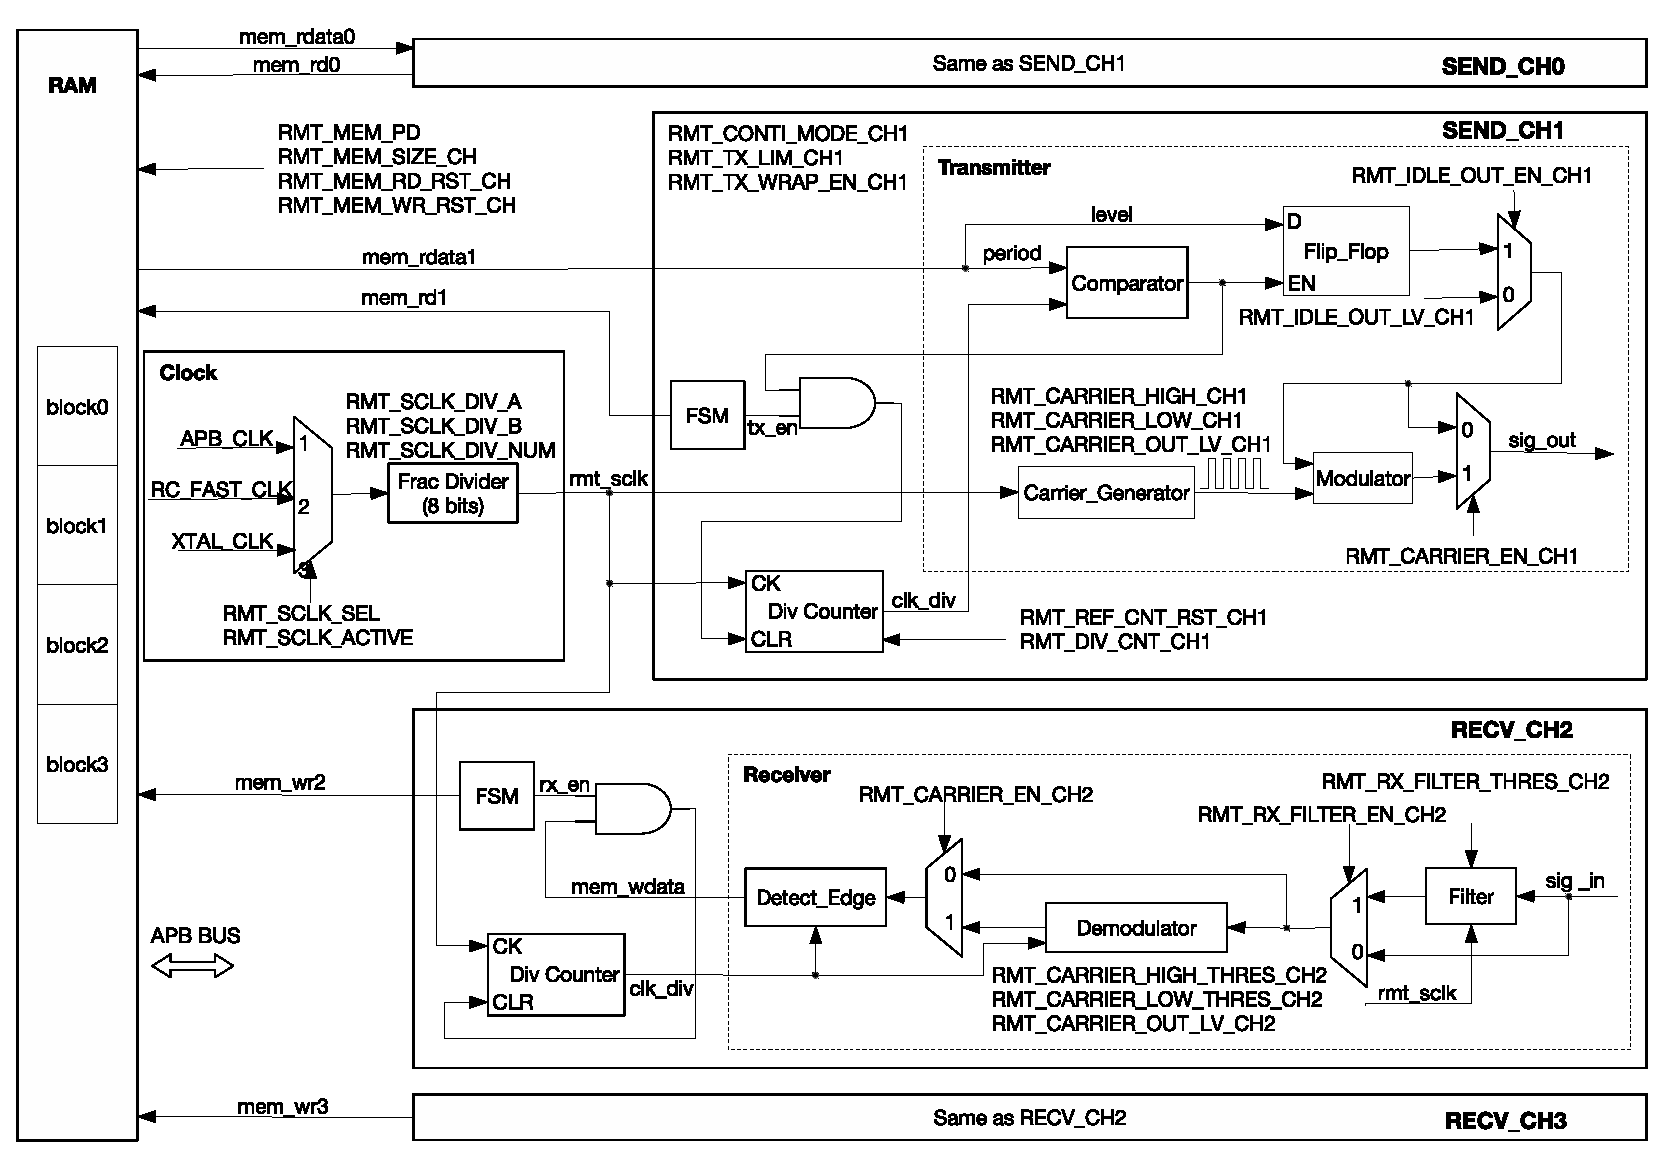
\includegraphics[width=1.0\textwidth]{./04-RMT/figures/rmt_architecture_20221213}
\centering
\caption{RMT 结构框图} \label{Figure:RMT2-1}
\end{figure}
RMT 模块有四个独立的通道，其中两个为发送通道，两个为接收通道。发送通道内部有各自的一个时钟分频计数器、状态机和发射器，接收通道内部有各自的一个时钟分频计数器、状态机和接收器。四个通道共享一块 192 x 32 bit 的 RAM。


\subsection{RMT RAM}
\begin{figure}[H]
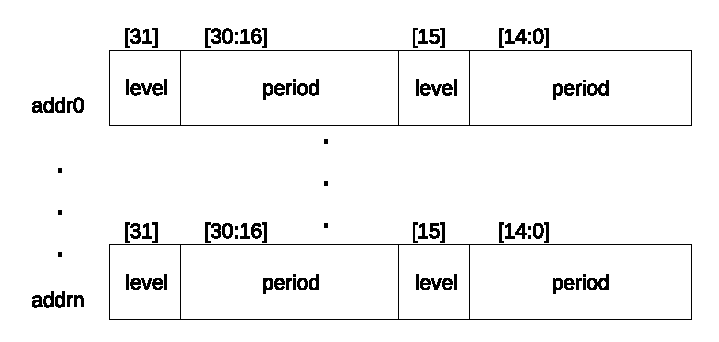
\includegraphics[width=0.5\textwidth]{./04-RMT/figures/rmt_data_structure.eps}
\centering
\caption{RAM中脉冲编码结构} \label{Figure:RMT2-2}
\end{figure}
RAM 中脉冲编码结构如图 \ref{Figure:RMT2-2} 所示。每个脉冲编码为 16 位，由 level 与 period 两部分组成。其中 level 表示输入或输出信号的逻辑电平值（0 或 1），period 表示该电平信号持续的时钟（图 \ref{Figure:RMT2-1} clk\_div）周期数。Period 为 0 是传输结束标志。非结束标志的 period 的数值需要满足与 APB 时钟和 RMT 时钟相关的限制条件：

\begin{equation}\label{eq:rmt-period-value}
5 \times T_{apb\_clk} + 6 \times T_{rmt\_sclk} < period \times T_{clk\_div}
\end{equation}

\begin{tiplisting}
RMT 时钟与 APB 时钟需满足以下关系：
    \begin{equation}
    1.5 \times T_{apb\_clk} < 9 \times T_{rmt\_sclk}
    \end{equation}
\end{tiplisting}

RAM 按照 48 x 32 位分成四个 block。默认情况下每个通道只能使用一个 block（固定为通道 0 使用 block 0，通道 1 使用 block 1，以此类推）。

当发送通道 \regindex{n} 或接收通道 \regindex{m} 单次传输的脉冲编码数大于一个 block 时，可以：
\begin{itemize}
    \item 置位 RMT\_MEM\_TX\_WRAP\_EN\_CH\regindex{n}/\regindex{m} 使能乒乓操作；
    \item 或通过配置 RMT\_MEM\_SIZE\_CH\regindex{n}/\regindex{m} 寄存器，允许该通道占用多个 block。
\end{itemize}

当设置 RMT\_MEM\_SIZE\_CH\regindex{n}/\regindex{m} > 1 时，通道 \regindex{n}/\regindex{m} 将占用 block (\regindex{n}/\regindex{m}) \verb+~+ block (\regindex{n}/\regindex{m} + RMT\_MEM\_SIZE\_CH\regindex{n}/\regindex{m} -1) 的存储空间。通道 \regindex{n}/\regindex{m} + 1 \verb+~+ \regindex{n}/\regindex{m} + RMT\_MEM\_SIZE\_CH\regindex{n}/\regindex{m} - 1 因为对应的 RAM block 被占用而无法使用。


注意，每个通道使用 RAM 的空间是根据地址从低到高进行映射的，因此通道 0 可以通过配置 RMT\_MEM\_SIZE\_CH0 寄存器来使用通道 1、 2、 3 的 RAM 空间，但是通道 3 不能使用通道 0、1 或 2 的 RAM 空间。因此 RMT\_MEM\_SIZE\_CH\regindex{n} 的最大值不应超过 (4 - \regindex{n})，RMT\_MEM\_SIZE\_CH\regindex{m} 的最大值不应超过 (2 - \regindex{m})。

RAM 可被 APB 总线及通道的发射器或接收器访问，为了防止接收通道访问 RAM 和 APB 访问 时发生冲突，用户可以通过配置 RMT\_MEM\_OWNER\_CH\regindex{m} 来决定当前 RAM 的使用权。当接收通道发生越权访问时会产生 RMT\_CH\regindex{m}\_OWNER\_ERR 标志信号。 

APB 总线访问 RAM 有 FIFO 和直接地址 (NONFIFO) 两种模式：
\begin{itemize}
    \item RMT\_FIFO\_MASK 置 1 时，选择直接地址模式；
    \item RMT\_FIFO\_MASK 置 0 时选择 FIFO 模式。
\end{itemize}

在 FIFO 模式下，APB 通过固定地址 \hyperref[regdesc:RMTCHNDATAREG]{RMT\_CH\regindex{n}/\regindex{m}DATA\_REG} 向 RAM 写数据或从 RAM 读数据。

在直接地址模式下，APB 向连续地址段写入数据，或从连续地址段读出数据。发送通道 \regindex{n} 对应的写地址段的首地址是：RMT 基地址 + 0x400 + \regindex{n}x48，第 2 个数据的访问地址是 RMT 基地址 + 0x400 + \regindex{n}x48 + 0x4，以此类推，后面的地址依次加上 0x4。接收通道 \regindex{m} 对应的读地址段的首地址是：RMT 基地址 + 0x460 + \regindex{m}x48，第 2 个数据的访问地址是 RMT 基地址 + 0x460 + \regindex{m}x48 + 0x4，以此类推，后面的地址依次加上 0x4。

当 RMT 模块不工作时，可以通过配置 \hyperref[fielddesc:RMTMEMFORCEPD]{RMT\_MEM\_FORCE\_PD} 寄存器使 RAM 工作于低功耗模式。

\subsection{时钟}\label{clock}
用户可以通过配置 RMT\_SCLK\_SEL 选择 RMT 的时钟源：APB\_CLK、RC\_FAST\_CLK 或 XTAL\_CLK，配置 RMT\_\\SCLK\_ACTIVE 为高电平来打开 RMT 的时钟。选择后的时钟经过小数分频得到 RMT 的工作时钟（图 \ref{Figure:RMT2-1} rmt\_sclk），分频系数为：

$$
RMT\_SCLK\_DIV\_NUM + 1 + RMT\_SCLK\_DIV\_A/RMT\_SCLK\_DIV\_B
$$

更多信息，请参考章节 \ref{mod:resclk} \textit{\nameref{mod:resclk}}。 RMT\_DIV\_CNT\_CH\regindex{n}/\regindex{m} 用于配置 RMT 通道内部的时钟分频器的分频系数，除 0 表示 256 分频外，其它分频数等同于 RMT\_DIV\_CNT\\\_CH\regindex{n}/\regindex{m} 的值。时钟分频器可以通过配置 RMT\_REF\_CNT\_RST\_CH\regindex{n}/\regindex{m} 进行复位。时钟分频器的分频时钟可供计数器使用。

\subsection{发射器}

\subsubsection{普通发送模式}

当 \hyperref[fielddesc:RMTTXSTARTCHN]{RMT\_TX\_START\_CH\regindex{n}} 置为 1 时，通道 \regindex{n} 的发射器开始从通道对应 RAM block 的起始地址，按照地址从低到高依次读取脉冲编码进行发送。当遇到结束标志（period 等于 0）时，发射器将结束发送返回空闲状态，并产生 \hyperref[int:RMTCHnTXENDINT]{RMT\_CH\regindex{n}\_TX\_END\_INT} 中断。配置 \hyperref[fielddesc:RMTTXSTOPCHN]{RMT\_TX\_STOP\_CH\regindex{n}} 可以使发射器立刻停止发送并进入空闲状态。发射器空闲状态发送的电平由结束标志中的 level 段或者是 \hyperref[fielddesc:RMTIDLEOUTLVCHN]{RMT\_IDLE\_OUT\_LV\_CH\regindex{n}} 决定。用户可以配置 \hyperref[fielddesc:RMTIDLEOUTENCHN]{RMT\_IDLE\_OUT\_EN\_CH\regindex{n}} 来选择这两种方式。这些配置都需要用置位 RMT\_CONF\_UPDATE\_CH\regindex{n} 的方法来更新进入发射器，详情见第 \ref{conf_update} 小节。



\subsubsection{乒乓发送模式}

当发送的脉冲编码较多时，可通过置位 \hyperref[fielddesc:RMTMEMTXWRAPENCHN]{RMT\_MEM\_TX\_WRAP\_EN\_CH\regindex{n}} 使能乒乓操作。在乒乓操作模式下，发射器会循环从通道对应的 RAM 区域取出脉冲编码进行发送，直至遇到结束标识为止。例如，当 \hyperref[fielddesc:RMTMEMSIZECHN]{RMT\_MEM\_\\SIZE\_CH\regindex{n}} = 1 时，发射器将从 48 * \regindex{n} 地址开始发送，然后对应 RAM 的地址递增。发完 (48 * (\regindex{n} + 1) - 1) 地址的数据后，下次继续从 48 * \regindex{n} 地址开始递增发送数据，依此类推，遇到结束标识时停止发送。\hyperref[fielddesc:RMTMEMSIZECHN]{RMT\_MEM\_SIZE\_CH\regindex{n}} > 1 的情形下，乒乓操作同样适用。

每当发射器发送的脉冲编码数大于等于 \hyperref[fielddesc:RMTTXLIMCHN]{RMT\_TX\_LIM\_CH\regindex{n}} 时，会产生 \hyperref[int:RMTCHnTXTHREVENTINT]{RMT\_CH\regindex{n}\_TX\_THR\_EVENT\_INT} 中断。在乒乓模式下，可以设置 \hyperref[fielddesc:RMTTXLIMCHN]{RMT\_TX\_LIM\_CH\regindex{n}} 为每个通道对应 RAM 空间的一半或几分之一。软件在检测到 \hyperref[int:RMTCHnTXTHREVENTINT]{RMT\_CH\regindex{n}\\\_TX\_THR\_EVENT\_INT} 中断之后，可以更新已使用过的 RAM 区域的脉冲编码，从而实现乒乓操作。

发送乒乓模式用到的 RMT\_MEM\_TX\_WRAP\_EN\_CH\regindex{n}、RMT\_MEM\_SIZE\_CH\regindex{n} 和 RMT\_TX\_LIM\_CH\regindex{n} 参数，都需要用置位 RMT\_CONF\_UPDATE\_CH\regindex{n} 的方法来更新进入发射器。详情见第 \ref{conf_update} 小节。

\subsubsection{发送加载波}

此外，发射器还可以对输出信号进行载波调制，置位 \hyperref[fielddesc:RMTCARRIERENCHN]{RMT\_CARRIER\_EN\_CH\regindex{n}} 可以使能该功能。载波的波形可配置。一个载波周期中高电平持续时间为 (\hyperref[fielddesc:RMTCARRIERHIGHCHN]{RMT\_CARRIER\_HIGH\_CH\regindex{n}} + 1) 个 rmt\_sclk 时钟周期，低电平持续的时间为 (\hyperref[fielddesc:RMTCARRIERLOWCHN]{RMT\_CARRIER\_LOW\_CH\regindex{n}} + 1) 个 rmt\_sclk 时钟周期。置位 \hyperref[fielddesc:RMTCARRIEROUTLVCHN]{RMT\_CARRIER\_OUT\_LV\_CH\regindex{n}} 时在输出信号高电平上加载波信号，清零 \hyperref[fielddesc:RMTCARRIEROUTLVCHN]{RMT\_CARRIER\_OUT\_LV\_CH\regindex{n}} 时在输出信号低电平上加载波信号。同时，在进行载波调制时，载波可以一直加载在输出信号上，也可以仅加载在有效的脉冲编码（RAM 中的数据）上。通过配置 \hyperref[fielddesc:RMTCARRIEREFFENCHN]{RMT\_CARRIER\_EFF\_EN\_CH\regindex{n}} 寄存器，可以选择这两种模式。RMT\_CARRIER\_EFF\_EN\_CH\regindex{n} 设置为 0 时在所有信号上加载波，设置为 1 时在有效信号上加载波。

上述载波调制中所需的配置参数，都需要用置位 RMT\_CONF\_UPDATE\_CH\regindex{n} 的方法来更新进入发射器，详情见第 \ref{conf_update} 小节。

\subsubsection{持续发送模式}

置位 RMT\_TX\_CONTI\_MODE\_CH\regindex{n} 可以使能发射器的持续发送模式。置位该寄存器后，发射器会循环发送 RAM 中的脉冲编码。持续发送模式下，如果遇到结束标志，会重新开始发送第一个数据；如果没有结束标志，会在发送到最后一个数据处回卷，再重新开始发送第一个数据。配置 RMT\_TX\_LOOP\_CNT\_EN\_CH\regindex{n} 后，发射器每遇到一次结束标志，循环发送的次数会加 1。当该次数达到 RMT\_TX \_LOOP\_NUM\_CH\regindex{n} 设定的值时，会产生 RMT\_CH\regindex{n}\_TX\_LOOP\_INT 中断。持续发送模式下，如果遇到的结束标志类型是 period[11:0] 为 0，那么这个结束标志前一个数据的 period 需要满足：

\begin{equation}
10 \times T_{apb\_clk} + 19 \times T_{rmt\_sclk} < period \times T_{clk\_div}
\end{equation}

而其它数据的 period，满足 \hyperref[eq:rmt-period-value]{非 0 period 关系式} 即可。

上述所需的配置参数，都需要用置位 RMT\_CONF\_UPDATE\_CH\regindex{n} 的方法来更新进入发射器，详情见第 \ref{conf_update} 小节。

\subsubsection{多通道同时发送}

首先配置 RMT\_TX\_SIM\_CH\regindex{n} 用于选择同步发送的通道，然后置位 RMT\_TX\_SIM\_EN 可以使能发射器多个通道同步发送的功能，将所选同步发送通道的 RMT\_TX\_START\_CH\regindex{n} 置为 1，当最后一个通道完成配置时，此时多个通道会同时启动发送。由于硬件条件的限制，两条通道不能保证完全同时开始发送，两条通道发送的时间间隔在 3 x T$_{clk\_div}$ 以内。RMT\_TX\_SIM \_EN 需要用置位 RMT\_CONF\_UPDATE\_CH\regindex{n} 的方法来更新进入发射器，详情见第 \ref{conf_update} 小节。



\subsection{接收器}

\subsubsection{普通接收模式}

RMT\_RX\_EN\_CH\regindex{m} 置为 1 时接收器开始工作，置为 0 时会停止接收。接收器会从信号的第一个跳变沿开始计数，并检测信号电平及其持续的时钟周期数，将其按照脉冲编码的格式存入 RAM 中。当信号在一个电平下持续的时钟周期数超过 RMT\_IDLE\_THRES\_CH\regindex{m} 时，接收器结束接收过程，返回空闲状态，并产生 RMT\_CH\regindex{m}\_RX\_END\_INT 中断。需要将 RMT\_IDLE\_THRES\_CH\regindex{m} 设置为超过接收电平的最大时钟周期数，否则会导致将正常的接收电平误判为进入空闲状态的后果。当接收数据存满了接收通道设置的 RAM 空间时，会停止接收，在非乒乓模式下会产生 \hyperref[int:RMTCHnERRINT]{RMT\_CH\regindex{m}\_ERR\_INT} 中断（由 RAM 满事件触发）。

上述所需的配置参数，都需要用置位 RMT\_CONF\_UPDATE\_CH\regindex{m} 的方法来更新进入接收器，详情见第 \ref{conf_update} 小节。

\subsubsection{乒乓接收模式}

当接收的脉冲编码较多时，可通过置位 RMT\_MEM\_RX\_WRAP\_EN\_CH\regindex{m} 使能通道 \regindex{m} 的乒乓操作。在乒乓操作模式下，接收器会将接收到的脉冲编码循环存入通道对应的 RAM 区域。当信号在一个电平下持续的时钟周期数超过 RMT\_IDLE\_THRES\_CH\regindex{m} 时，接收器结束接收过程，返回空闲状态，并产生 RMT\_CH\regindex{m}\_RX\_END\_INT 中断。例如，当 RMT\_MEM\_SIZE\_CH\regindex{m} = 1 时，接收器将从 48 * \regindex{m} 地址开始接收，然后对应 RAM 的地址递增。收完 (48 * (\regindex{m} + 1) - 1) 地址的数据后，下次继续从 48 * \regindex{m} 地址开始递增接收数据，以此类推，遇到信号在一个电平下持续的时钟周期数超过 RMT\_IDLE\_THRES\_CH\regindex{m} 时停止接收。RMT\_MEM\_SIZE\_CH\regindex{m} > 1 的情形下，乒乓操作同样适用。

每当接收器接收的脉冲编码数大于等于 RMT\_RX\_LIM\_CH\regindex{m} 时，会产生
RMT\_CH\regindex{m}\_RX\_THR\_EVENT\_INT 中断。在乒乓模式下，可以设置 RMT\_RX\_LIM\_CH\regindex{m}
为每个通道对应 RAM 空间的一半或几分之一。软件在检测到 RMT\_CH\regindex{m}\_RX\_THR\_EVENT\_INT
中断之后，可以回收已使用过的 RAM 区域的脉冲编码，从而实现乒乓操作。

上述所需的配置参数，都需要用置位 RMT\_CONF\_UPDATE\_CH\regindex{m} 的方法来更新进入发射器，详情见第 \ref{conf_update} 小节。



\subsubsection{接收滤波}

每个通道都可以通过置位 RMT\_RX\_FILTER\_EN\_CH\regindex{m} 使能接收器对输入信号进行滤波的功能。滤波器的功能为连续采样输入信号，如果输入信号在连续 RMT\_RX\_FILTER \_THRES\_CH\regindex{m} 个 rmt\_sclk 时钟周期内保持不变，则输入信号有效，否则输入信号无效。只有有效的输入信号才能通过滤波器。因此，滤波器会滤除脉冲宽度小于 RMT\_RX\_FILTER\_THRES\_CH\regindex{n} 个 rmt\_sclk 时钟周期的线路毛刺。

上述所需的配置参数，都需要用置位 RMT\_CONF\_UPDATE\_CH\regindex{m} 的方法来更新进入发射器，详情见第 \ref{conf_update} 小节。

\subsubsection{接收去载波}

此外，接收器还可以对输入信号或滤波后的输出信号进行去载波调制，置位 RMT\_CARRIER\_EN\_CH\regindex{m} 可以使能该功能。
去载波分为去除高电平载波和低电平载波两种类型：
\begin{itemize}
    \item 置位 RMT\_CARRIER\_OUT\_LV\_CH\regindex{m}，设置去除高电平载波;
    \item 清零 RMT\_CARRIER\_OUT\_LV\_CH\regindex{m}，设置去除低电平载波。
\end{itemize}

配置 RMT\_CARRIER\_HIGH\_THRES\_CH\regindex{m} 和 RMT\_CARRIER\_LOW\_THRES\_CH\regindex{m}  来设置去载波的高电平阈值和低电平阈值。当信号的高电平持续时间小于 RMT\_CARRIER\_HIGH\_THRES\_CH\regindex{m} 个 clk\_div 分频时钟周期，或者信号的低电平持续时间小于 RMT\_CARRIER\_LOW \_THRES\_CH\regindex{m} 个 clk\_div 分频时钟周期，就会被认为是载波被滤除。

上述所需的配置参数，都需要用置位 RMT\_CONF\_UPDATE\_CH\regindex{m} 的方法来更新进入接收器，详情见第 \ref{conf_update} 小节。

\subsection{配置参数更新}\label{conf_update}
RMT 的配置寄存器均需要配置各自通道的 RMT\_CONF\_UPDATE\_CH\regindex{n}/\regindex{m} 寄存器位来更新进入各自通道，更新方法是向 RMT\_CONF\_UPDATE\_CH\regindex{n}/\regindex{m} 写入高电平。发送通道和接收通道需要通过这种方法更新的配置参数列在下表中。

\begin{longtable}{ | p{6cm} | p{7cm} | }
\caption{更新配置参数}
\label{tab:rmt-config-update}\\
\hline
    \rowcolor{lightgray}
        \textbf{配置寄存器} & \textbf{配置参数}  \\ \hline
    \endfirsthead
    
    \multicolumn{2}{c}{\bfseries \tablename\ \thetable{} -- 接上页}\\\hline

    \rowcolor{lightgray}
        \textbf{配置寄存器} & \textbf{配置参数}  \\ \hline
    \endhead
    \multicolumn{2}{r}{\textbf{见下页}} \\
        \endfoot
        \endlastfoot
        \hline
        
\multicolumn{2}{|c|}{\textbf{发送通道}} \\ \hline
\multirow{8}{*}{\hyperref[regdesc:RMTCHNCONF0REG]{RMT\_CH\regindex{n}CONF0\_REG}}  &   RMT\_CARRIER\_OUT\_LV\_CH\regindex{n}    \\ \cline{2-2} 
                   & RMT\_CARRIER\_EN\_CH\regindex{n}      \\ \cline{2-2} 
                   &  RMT\_CARRIER\_EFF\_EN\_CH\regindex{n}     \\ \cline{2-2} 
                   & RMT\_DIV\_CNT\_CH\regindex{n}      \\ \cline{2-2}
                   & RMT\_TX\_STOP\_CH\regindex{n}      \\ \cline{2-2}
                   & RMT\_IDLE\_OUT\_EN\_CH\regindex{n}      \\ \cline{2-2}
                   & RMT\_IDLE\_OUT\_LV\_CH\regindex{n}      \\ \cline{2-2}
                   & RMT\_TX\_CONTI\_MODE\_CH\regindex{n}      \\ \hline
\multirow{2}{*}{RMT\_CH\regindex{n}CARRIER\_DUTY\_REG}  &   RMT\_CARRIER\_HIGH\_CH\regindex{n}    \\ \cline{2-2} 
                   & RMT\_CARRIER\_LOW\_CH\regindex{n}      \\ \hline
\multirow{3}{*}{RMT\_CH\regindex{n}\_TX\_LIM\_REG}  &   RMT\_TX\_LOOP\_CNT\_EN\_CH\regindex{n}    \\ \cline{2-2} 
                   &   RMT\_TX\_LOOP\_NUM\_CH\regindex{n}    \\ \cline{2-2} 
                   & RMT\_TX\_LIM\_CH\regindex{n}     \\ \hline
RMT\_CH\regindex{n}\_TX\_SIM\_REG & RMT\_TX\_SIM\_EN \\ \hline

\multicolumn{2}{|c|}{\textbf{接收通道}} \\ \hline
\multirow{4}{*}{RMT\_CH\regindex{m}CONF0\_REG}  &   RMT\_CARRIER\_OUT\_LV\_CH\regindex{m}    \\ \cline{2-2} 
                   &   RMT\_CARRIER\_EN\_CH\regindex{m}    \\ \cline{2-2} 
                    &   RMT\_IDLE\_THRES\_CH\regindex{m}    \\ \cline{2-2} 
                   & RMT\_DIV\_CNT\_CH\regindex{m}     \\ \hline
\multirow{2}{*}{RMT\_CH\regindex{m}CONF1\_REG}  &   RMT\_RX\_FILTER\_THRES\_CH\regindex{m}    \\ \cline{2-2} 
                   & RMT\_RX\_EN\_CH\regindex{m}     \\ \hline
\multirow{2}{*}{RMT\_CH\regindex{m}\_RX\_CARRIER\_RM\_REG}  &   RMT\_CARRIER\_HIGH\_THRES\_CH\regindex{m}    \\ \cline{2-2} 
                   & RMT\_CARRIER\_LOW\_THRES\_CH\regindex{m}     \\ \hline

RMT\_CH\regindex{m}\_RX\_LIM\_REG & RMT\_RX\_LIM\_CH\regindex{m} \\ \hline

RMT\_REF\_CNT\_RST\_REG & RMT\_REF\_CNT\_RST\_CH\regindex{m} \\ \hline
\end{longtable}

\subsection{中断}
\begin{itemize}
\item \label{int:RMTCHnERRINT}RMT\_CH\regindex{n}/\regindex{m}\_ERR\_INT：当通道 \regindex{n}/\regindex{m} 发生读写数据不正确，或内存空满错误时，即触发此中断。    
\item \label{int:RMTCHnTXTHREVENTINT}RMT\_CH\regindex{n}\_TX\_THR\_EVENT\_INT：发射器每发送 \hyperref[regdesc:RMTCHNTXLIMREG]{RMT\_CH\regindex{n}\_TX\_LIM\_REG} 的数据，即触发一次此中断。
\item \label{int:RMTCHmRXTHREVENTINT}RMT\_CH\regindex{m}\_RX\_THR\_EVENT\_INT：接收器每接收 \hyperref[regdesc:RMTCHMRXLIMREG]{RMT\_CH\regindex{m}\_RX\_LIM\_REG} 的数据，即触发一次此中断。
\item \label{int:RMTCHnTXENDINT}RMT\_CH\regindex{n}\_TX\_END\_INT：当发射器停止发送信号时，即触发此中断。
\item \label{int:RMTCHnRXENDINT}RMT\_CH\regindex{m}\_RX\_END\_INT：当接收器停止接收信号时，即触发此中断。
\item \label{int:RMTCHnTXLOOPINT}RMT\_CH\regindex{n}\_TX\_LOOP\_INT：发射器处于循环发送模式时，当循环次数达到 \hyperref[fielddesc:RMTTXLOOPNUMCHN]{RMT\_TX\_LOOP\_NUM\_CH\regindex{n}} 的值后，会产生此中断。
\end{itemize}


%%%%%%%%%%%%%%%%%%%%%%%%
%%% Register Summary %%%
%%%%%%%%%%%%%%%%%%%%%%%%

% >>> Update the sample text below and insert
%     the info on register summary into the subfile <<<

\clearpage
\section{寄存器列表}
\label{sec:rmt-reg-summ}
\hypertarget{rmt-reg-summ}{}

本小节的所有地址均为相对于 RMT 基地址的地址偏移量（相对地址），具体基地址请见章节 \ref{mod:sysmem} \textit{\nameref{mod:sysmem}} 中的表 \ref{tab:sysmem-base-address}。

请查看章节 \hyperref[glossary-access-types]{\textit{寄存器的访问类型}}，了解“访问”列缩写的含义。

\subfile{\modulefiles/rmt_reg_726new_summary_cn}


%%%%%%%%%%%%%%%%%
%%% Registers %%%
%%%%%%%%%%%%%%%%%

% >>> Update the sample text below and insert
%      the info on registers into the subfile <<<


\section{寄存器}

本小节的所有地址均为相对于 RMT 基地址的地址偏移量（相对地址），具体基地址请见章节 \ref{mod:sysmem} \textit{\nameref{mod:sysmem}} 中的表 \ref{tab:sysmem-base-address}。

\subfile{\modulefiles/rmt_reg_726new_cn}


\end{document}
